\chapter{Results}\label{chp:results}

What happens in this chapter?

Recapitulate the predictions for reaction times
\section{Descriptive Statistics} \label{sec:desc_stats}

For both raw and log-transformed reaction times, t-tests confirmed that the difference in means between groups was not due to random chance ($p$<0.05). All of the previous observations, summarised in \ref{fig:boxplot} below, paint a clear picture: compared to inflectional forms, members of the derivational diminutive category elicit slightly faster reaction times on average. Given the predictions recapitulated above, this is a \textbf{X} observation.
\begin{figure}[h]
    \centering
    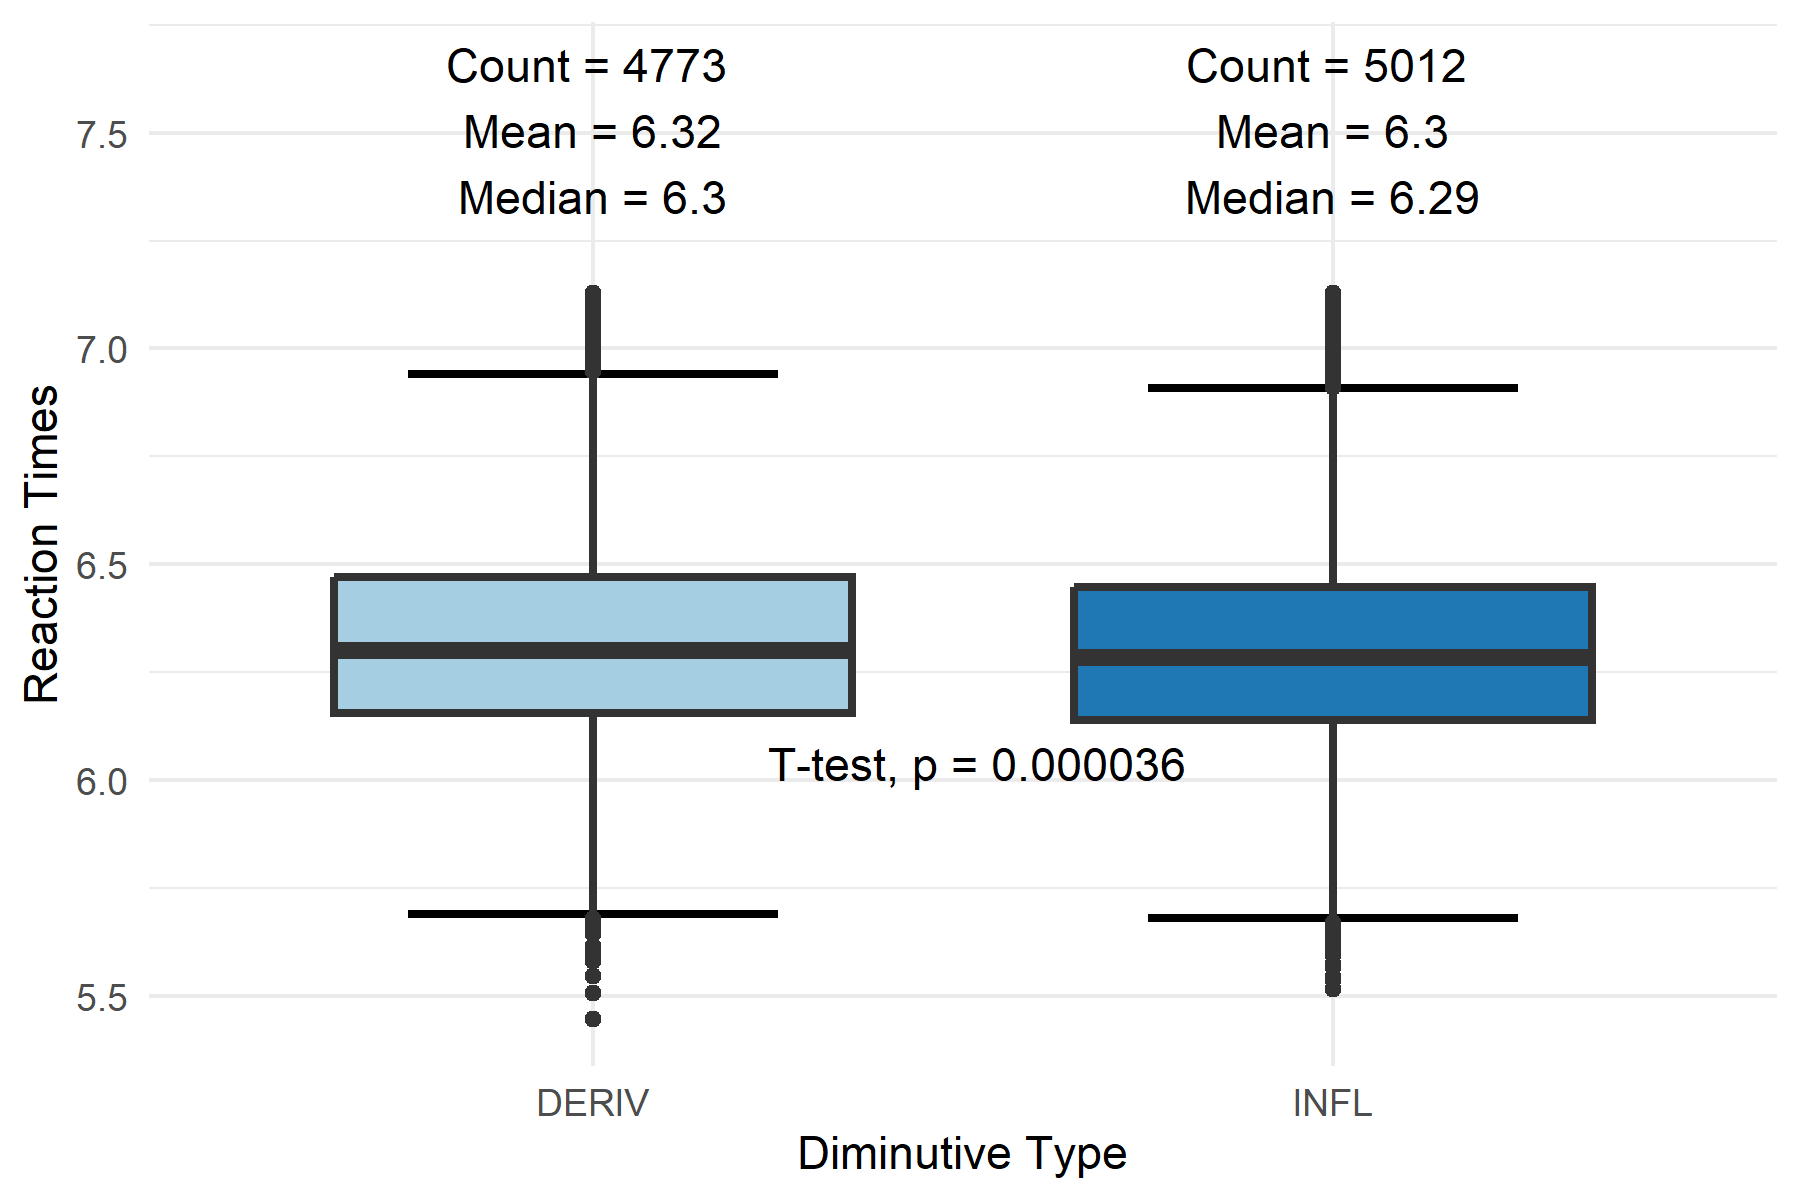
\includegraphics[width=\textwidth]{images/dim_box.png}
    \caption[Boxplot of log-transformed reaction times by diminutive type]{Boxplot of log-transformed reaction times by diminutive type. 50\% of all observations fall within the interquartile range (IQR) represented by each box; the thick lines stand for median values. Values beyond the box represent the top and bottom 25\%. The distance between each whisker and its side of the box equals 1.5*IQR; more extreme values are represented by dots beyond each whisker. Summary information is provided above each condition; difference between means is attested as significant by way of a t-test ($p$<0.05).}
    \label{fig:boxplot}
\end{figure}

\section{Inferential Statistics} \label{sec:inf_stats}
A mixed-effects linear regression model was chosen as the most suited to the data structure. The final formula for the experimental model is presented in (\ref{ex:modelformula}). All continuous predictors were standardised and centered. This homogenises effect sizes by putting the intercept of each predictor at its mean, with every data point's distance from it being measured in standard deviations. In practical terms, this allows for easier comparison of the fixed effects in Table \ref{tab:reg-fixed}: for every predictor except \texttt{dim\_type}, the reported effect size is the change in reaction times per 1 standard deviation above the mean. The contrasts between the values of \texttt{dim\_type} were sum-coded and \texttt{deriv} was chosen as the positive value; the reported effect for diminutive type therefore reflects the predicted change in reaction times under the derivational condition.

\begin{exe}
\ex \label{ex:modelformula}
\texttt{RT \textasciitilde ~dim\_type*frequency + nmorph + orth. similarity \\ 
+ concreteness + age of acquisition + word prevalence \\
+ (1|participant) + (1|item)}
\end{exe}

The complete final model explains 42.6\% of the total variance (conditional $R^2$=0.4261). However, random effects make the largest contribution by far: only 6\% of total variance is explained by the fixed effects in the model (marginal $R^2$=0.0616), indicating the importance of the by-participant and by-item intercepts. Table \ref{tab:reg-fixed} summarises model predictions for fixed effects; random effects are summarised in Table \ref{tab:reg-random}. The individual effect of each predictor is explained in its respective subsection below.

\begin{table}[h]
\centering
\label{tab:reg-fixed}
\resizebox{0.8\textwidth}{!}{%
\begin{tabular}{lccc}
\toprule
\textbf{Predictor} & \textbf{Estimate} & \textbf{Standard Error} & \textbf{$p$-Value}  \\ \midrule
(Intercept) & 6.3137 & 0.0161 & <0.001\\
Diminutive Type & -0.0032 & 0.0036 & 0.3669 \\
\textbf{Frequency}  & -0.0245 & 0.0045 & \textbf{<0.001} \\
Morpheme Count & 0.0026 & 0.0051 & 0.6089 \\
\textbf{Orth. Similarity} & 0.0202 & 0.0052 & \textbf{<0.001} \\
Concreteness & 0.0020 & 0.0038 & 0.5962 \\
\textbf{Age of Acquisition} & 0.0168 & 0.0043 & \textbf{<0.001} \\
\textbf{Word Prevalence} & -0.0471 & 0.0085 & \textbf{<0.001} \\
\textbf{Dim. Type*Frequency} & 0.0071 & 0.0032 & \textbf{0.0298} \\
\bottomrule
\end{tabular}%
}
\caption[Summary of fixed effects from the experimental model]{Summary of fixed effects from the experimental model. All continuous predictors centered and standardised, categorical predictor \textit{Diminutive Type} sum-coded, predictors the effects of which have achieved significance ($p$<0.05) have their names and $p$-values in boldface.}
\end{table}

\subsection{Diminutive Type} \label{subsec:dimtype}
The predictions for diminutive type are replicated in the model, as there is an observable predicted change in estimate depending on the type of diminutive. While derived wordforms are predicted to require less time to recognise, the predictor is not statistically significant on its own, and its effect size is miniscule. However, due to the presence of an interaction term in the model, the effect of diminutive type is not interpretable on its own; diminutive type and frequency are conditioned on each other, and their effects need to be interpreted together (\citeauthor{Winter+2019} \citeyear{Winter+2019}). See Subsection \ref{subsec:interaction} below for an interpretation of the interaction.
\subsection{Frequency} \label{subsec:freq}
Frequency is historically one of the most robust predictors in lexical recognition studies (\citeauthor{Brysbaert+etal+2016} \citeyear{Brysbaert+etal+2016}). Higher surface frequency is consistently associated with lower reaction times, as more frequently used words are postulated to require less time for lexical activation. These particular frequency values are based on an expanded version of the subtitle corpus SUBTLEX-NL (\citeauthor{Keuleers+etal+2010} \citeyear{Keuleers+etal+2010}). In addition, the values have been Zipf-transformed to arrive at a standardized frequency measure independent of corpus size (\citeauthor{vanHeuven+etal+2014} \citeyear{vanHeuven+etal+2014}). A Zipf value of 1 corresponds to an approximate word frequency of 1 per 100 million words, a value of 2 corresponds to 1 per 10 million, and so on. Higher Zipf values therefore reflect higher word frequencies and are predicted to elicit lower reaction times. This prediction holds up in our model, with Zipf-tansformed frequency being a facilitating factor with one of the largest effect sizes in the whole model. Again, because of the interaction term, the effect of frequency cannot be interpreted independently from diminutive type.
\subsection{Morpheme Count} \label{subsec:nmorph}
The number of morphemes is an approximate measurement for a wordform's internal complexity. While the values assigned to each wordform are theory-specific, the general prediction under the assumption of full decomposition is the same: more internally complex words require longer to decompose into constituent morphemes, look those morphemes up, recombine them into the wordform in question, and check for well-formedness. This prediction is upheld in the experimental model; however, while the variable is predicted to be inhibitory, the effect size is rather negligible, and the predictor does not make a statistically significant contribution to the model. \textbf{FIND CITATION FOR THIS}
\subsection{Orthographic Similarity} \label{subsec:old20}
Orthographic similarity is a measure of how similar a word is to its immediate orthographic neighbours as determined by a set inventory of possible permutations such as letter substitution and/or transposition, addition or subtraction. While there exist multiple ways of quantifying neighbourhood effects, the one chosen for this analysis is the orthographic Levenshtein distance based on the closest 20 words (OLD20, \citeauthor{Yarkoni+etal+2008} \citeyear{Yarkoni+etal+2008}). Higher OLD20 ratings reflect the average number of permutations needed to transform a wordform into one of its 20 closest neighbours, and the higher the rating, the less similar the wordform is to its neighbours. The attested effect of OLD20 is therefore inhibitory (\citeauthor{Brysbaert+etal+2016} \citeyear{Brysbaert+etal+2016}, among others), as more dissimilar items take longer to recognize. The model above replicates the prediction: OLD20 is a statistically significant predictor with a sizeable inhibitory effect.
\subsection{Concreteness} \label{subsec:concreteness}
A predictor adopted from \citeauthor{Brysbaert+etal+2014} (\citeyear{Brysbaert+etal+2014}), concreteness quantifies the degree to which a given wordform refers to a perceivable entity, e.g. a object in the real world compared to an abstract concept. It is represented on a 5-point scale and based on averaged subjective ratings collected from 75 students at the University of Leuven. According to \citeauthor{Brysbaert+etal+2014} (\citeyear{Brysbaert+etal+2014}), more concrete words are predicted to require less time to recognize. However, \citeauthor{Brysbaert+etal+2016} (\citeyear{Brysbaert+etal+2016}) report a reverse effect of concreteness, with less concrete words predicting lower reaction times. They attempt to explain this inversion through the typically higher emotional load of more abstract wordforms compared to their more concrete counterparts: strongly positive or negative wordforms induce quicker responses. While the model above reflects the inverted prediction as reported in \citeauthor{Brysbaert+etal+2016} (\citeyear{Brysbaert+etal+2016}), the predictor is not statistically significant, and its effect size is the lowest in the entire model.
\subsection{Age of Acquisition} \label{subsec:aoa}
Another predictor based on subjective ratings from students is the age of acquisition (AoA), similarly adopted from \citeauthor{Brysbaert+etal+2014} (\citeyear{Brysbaert+etal+2014}). Despite the name, it does not reflect the actual average age when the wordform is acquired, and functions instead as an estimate of processing cost: in the process of value assignment, a word is given an age of acquisition rating based on how (self-reportedly) easy it is to understand it, the rationale being something like "this is an easy word; thus, I must have learned it early" (\citeauthor{Brysbaert+etal+2016} \citeyear{Brysbaert+etal+2016}:23). Higher AoA values therefore predict longer reaction times and are replicated as such in the model: the predictor is statistically significant and its effect size is relatively substantial.
\subsection{Word Prevalence} \label{subsec:prevalence}
A novel explanatory variable proposed by \citeauthor{Keuleers+etal+2015} (\citeyear{Keuleers+etal+2015}) and introduced in the Dutch Lexicon Project 2 dataset, word prevalence is defined as "word knowledge in the population" (\citeauthor{Brysbaert+etal+2016} \citeyear{Brysbaert+etal+2016}) and intended as a supplementary predictor to word frequency. According to \citeauthor{Brysbaert+etal+2016}, frequency is corpus-dependent and is not always the most reliable measure of how well-known or widely-used a wordform is: for example, words referring to household objects are well-known in the general population, but this fact is not represented in their (typically low) frequency scores. Word prevalence was introduced to account for this as well as other predictive shortcomings of frequency. Its prediction is straightforward: the better-known a word, the less time it takes to recognise. The values for prevalence were collected by \citeauthor{Keuleers+etal+2015} from over 100.000 Dutch-speaking participants from Flanders. Both \citeauthor{Keuleers+etal+2015} (\citeyear{Keuleers+etal+2015}) and \citeauthor{Brysbaert+etal+2016} (\citeyear{Brysbaert+etal+2016}) report the predictor as one of the most correlated with reaction times, usually second-best after (and in some cases even more explanatory than) frequency. As such, it is no surprise to see this effect replicated in a model based on a subset of the DLP2: word prevalence is a facilitatory explanatory variable with the single largest effect size in the entire model.
\subsection{Interaction of Diminutive Type and Frequency} \label{subsec:interaction}
The interaction of frequency with diminutive type reveals an unexpected pattern: derived forms are generally predicted to elicit faster responses than inflected ones, yet the relationship is flipped for particularly frequent members. In general, frequency has a facilitatory effect, speeding up visual recognition for both groups, but its effect is much stronger for inflected items. As visualised in Figure \ref{fig:interaction}, somewhere between the Zipf-values of 5 (1 per 10.000 words) and 6 (1 per 1000 words), inflected forms start eliciting lower reaction times than derived ones. This observation is more in line with the difference in means observed in the boxplot. While the predicted effect size reported in the model is an order of magnitude lower than those of other statistically significant predictors, it still falls within the parameters of statistical significance ($p$<0.05).
\begin{figure}[h]
    \centering
    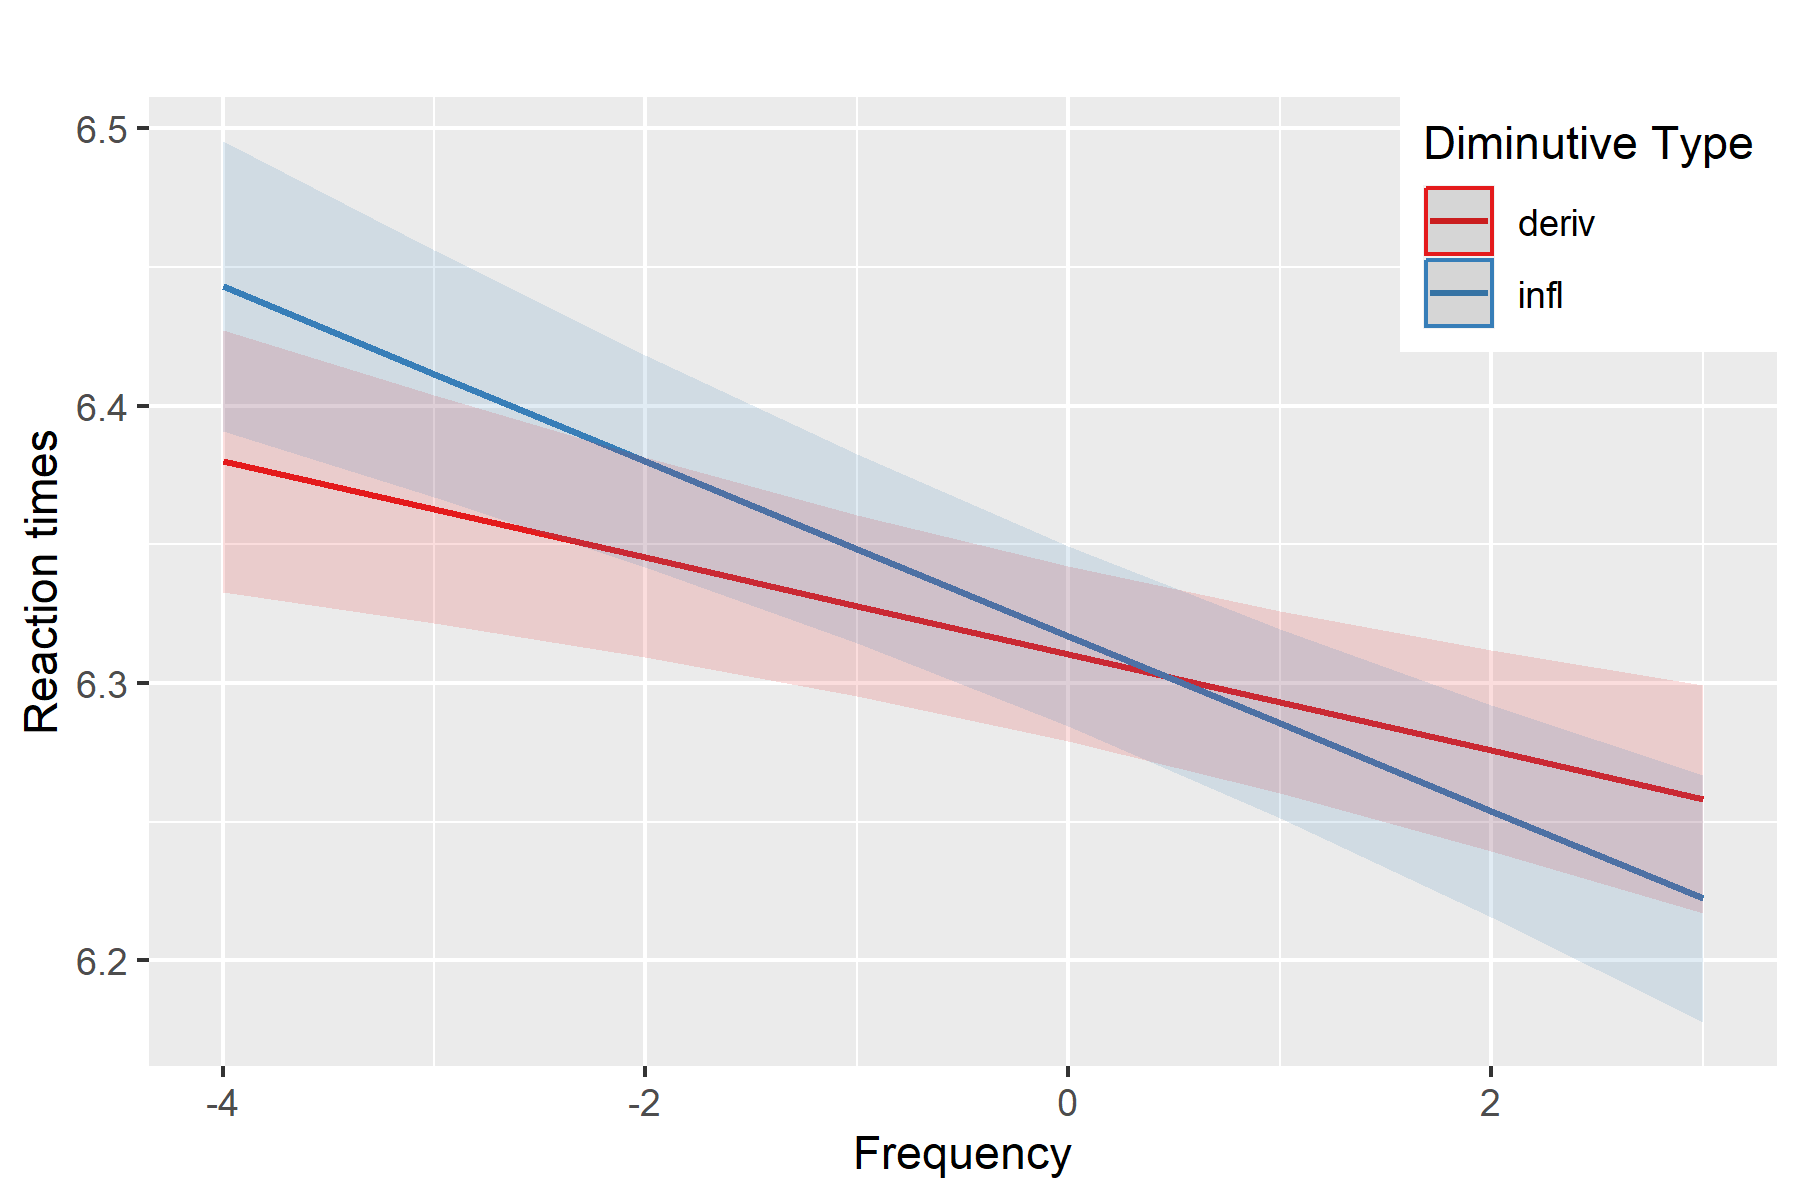
\includegraphics[width=\textwidth]{images/mod_int.png}
    \caption[Frequency interactions from the experimental model]{Frequency interactions from the experimental model. Both measurements on the X and Y axis are reported post-transformation: logarithmic for reaction times and Zipf-transformation for frequency. Zipf-values subsequently centered for easier interpretation of effects in the model; 0 stands for Zipf-value of 5, i.e. 1 occurrence per 10.000 words.}
    \label{fig:interaction}
\end{figure}
\subsection{Random Effects}
The random effects were included in the model to satisfy the assumption of every data point being independent from the rest, resulting in the addition of varying intercepts by participant ($N$=81) and item ($N$=270). Table \ref{tab:reg-random} presents a summary of random effects. As is typical (\cite{Winter+2019}), intercepts by participant account for more variance in the data compared to intercepts by item. Nevertheless, there is some considerable residual variance left unexplained in the model.
\begin{table}[h]
\centering
\label{tab:reg-random}
\resizebox{0.8\textwidth}{!}{%
\begin{tabular}{lccc}
\toprule
\textbf{Groups} & \textbf{Group Size} & \textbf{Variance} & \textbf{Standard Deviation}  \\ \midrule
item & 270 & 0.0018 & 0.0426\\
participant & 81 & 0.0202 & 0.1422 \\
residual & \textemdash & 0.0347 & 0.1863 \\
\bottomrule
\end{tabular}%
}
\caption[Summary of random effects from the experimental model]{Summary of random effects from the experimental model.}
\end{table}

\section{Summary} \label{sec:stats_summary}
\begin{itemize}
\item Sum up all facts, no opinion on the facts
\end{itemize}
